\chapter{Einleitung}
Das Schlüsselelement einer Website, das dem Nutzer die Interaktionen mit dem System ermöglicht oder verwehrt, ist das User Interface (UI).
Schlecht verständliche UIs können sich schlecht auf die Verwendung eines guten Systems auswirken. \cite[S.30]{Am-dUI}
%personalisierte Services einführen
Die Idee hinter adaptiven UIs ist, ein User Interface für einen möglichst breiten Personenkreis, optimal zugänglich zu gestalten.
Momentan gestaltet es sich schwer Interfaces an die Bedürfnisse einzelner Nutzer anzupassen und den Kontext der Nutzung zu berücksichtigen.
Deswegen gehen viele UIs nur vereinzelt auf die individuellen Bedürfnisse des Nutzers und den Kontext der Software ein.
%Das User Interface (UI) einer Software ist das Schlüsselelement, dass dem Nutzer die Interaktion mit den  Funktionen einer Software ermöglicht oder verwehrt. Ist ein UI für den Nutzer nicht verständlich,  kann sich dies negativ auf die Verwendung einer gut geschrieben Software auswirken. [Vgl. P. A. Akiki, A. K. Bandara und Y. Yu (2014): Adaptive model-driven user interface development systems, ACM Computing Surveys 47, 1, Artikel 9, S. 33, URL: http://dx.doi.org/10.1145/2597999]

%Einige der bisherigen Design Ansätze für die Gestaltung von UIs, wie „Universal Design“ [Vgl. R. L. Mace, G. e J. Hardie und J. P. Place (1990): Accessible Environments: Toward Universal Design, In Design Intervention: Toward a More Humane Architecture, Center for Accessible Housing, North Carolina State University],  „Inclusive Design“ [Vgl. S. Keates, P. J. Clarkson, L.-A. Harrison und P. Robinson (2000): Towards a Practical Inclusive Design Approach, In Proceedings on the 2000 Conference on Universal Usability, ACM, S. 45–52]  und „Design for All“ [Vgl. C. Stephanidis (1997): Towards the Next Generation of UIST: Developing for all Users, In Proceedings of the 7th International Conference on Human-Computer Interaction (HCI’97), Elsevier Science Inc., S. 473–476] folgen dem Konzept, ein UI für einen möglichst breiten Personenkreis, optimal zugänglich zu gestalten. 

%Dieser Gedanke ist erst einmal per se nicht falsch, da es sich mit bisherigen Methoden eher schwer gestaltet Interfaces auf die Bedürfnisse einzelner Nutzer abzustimmen und den Kontext der Nutzung zu berücksichtigen. Deshalb gehen bisher viele UIs nur vereinzelt auf die individuellen Bedürfnisse des Nutzers und den Benutzungskontext der Software ein. 
Oftmals geschieht dies durch zusätzliche individuelle Anpassungen durch den Nutzer (Adaptierbarkeit des UIs),
d.h. das Interface lässt sich in einem bestimmten Rahmen nach den Wünschen des jeweiligen Nutzers anpassen.
Dabei entstehen durch die zunehmende Rechenleistung und den vermehrten Einsatz von Sensoren in mobilen Geräten
(Smartphones, Tablets, Wearables) neue Möglichkeiten UIs mit faktorenabhängigen Funktionalitäten auszustatten.
Somit können viele unterschiedliche UIs einer Software entstehen, die den individuellen Nutzer bei der Verwendung der Software unterstützen.
Diese Nutzeroberflächen werden Adaptive User Interfaces genannt. Forschungen aus dem Bereich der Informatik liefern Ergebnisse die zeigen,
dass es Möglich ist, dass sich Software User Interfaces nicht nur dem Kontext sondern auch dem individuellen Nutzer anpassen können. [Vgl. K. Gajos(2008): Automatically Generating Personalized User Interfaces, A dissertation submitted in partial fulfillment of the requirements for the degree of Doctor of Philosophy, Computer Science and Engineering, University of Washington, Seattle, WA, USA]
Bei diesen adaptiven Systemen wird davon ausgegangen, dass sich die Usability der Software durch die Anpassung an die
variablen Nutzerbedürfnisse und den Kontext verbessert.

Once the AUI records the events of humancomputer interaction and discovers patterns of user behavior, it can provide just-in-time assistance by
predicting a user’s most likely plan and then performing part of the plan on the user’s behalf. It also manipulates the software system semiautonomously,
thus reducing the intervention required.

\section{Problemstellung}
Bei dem Erstellen von Benutzeroberflächen gibt es drei Herausforderungen zu beachten:
\begin{itemize}
    \item unerwünschte Eingriffe in die Benutzererfahrung
    \item Komplexität der Implementierung
    \item robuste User Interfaces
\end{itemize}

\begin{figure}[h]
    \centering
    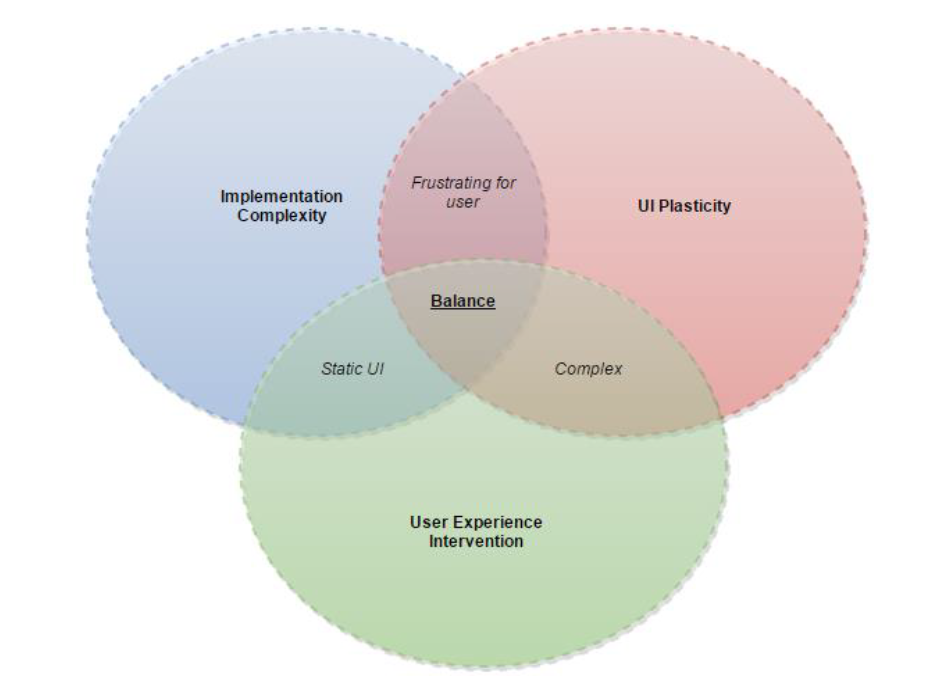
\includegraphics[height=.65\textwidth]{implChallenges.png}
    \caption{Die drei Herausforderungen und ihre Schnittstellen}
\end{figure}

\subsection{Schlechte Benutzererfahrung}
Ein UI mit mehreren adaptiven Komponenten kann den Nutzer verwirren und zusätzlich können automatische
und häufige Änderungen an diesen Komponenten dem Nutzer das Gefühl geben, er habe die Kontrolle verloren.

Das Problem mit \textbf{mehreren adaptiven Komponenten} ist, dass wenn sich die Komponenten
(und somit auch UI) ändern, der Nutzer sich nicht mehr zurecht findet und aus seiner comfort
zone gebracht wird. Dabei ist es nicht entscheidend, wie gut die zugrunde liegende Intelligenz ist,
die die Entscheidungen über die Änderung der adaptiven Komponenten trifft.

Aus Sicht des Benutzers kann das Gefühl von Kontrollverlust zu Verwirrung, Stress und sogar Frustration führen. So toll
\begin{itemize}
    \item eine dropdown Liste, die seine Optionen selbst filtert, wenn zu viele Daten vorhanden sind,
    \item eine Tabelle die sich je nach Input-Typ sortiert oder
    \item Pop-Ups, die die nächsten Aktionen eines Nutzers vorhersagen und / oder eine Vorauswahl an Aktionen für einen machen,
\end{itemize}
sind, wenn sie alle gleichzeitig in einer Webanwendung existieren führt das zu einer schlechten Benutzererfahrung.

Den Nutzer um eine \textbf{Bestätigung} bitten, wenn ein Passwort eingegeben wird oder wenn gesicherte Daten
überschrieben werden oder beim Absenden einer Email oder Form ist sehr wichtig.
Diese Pop-Ups sollten sehr vorsichtig und nutzerzentriert gewählt werden. Der Grad zwischen einem
angenehmen und irritierenden Pop-Up Fenster ist sehr schmal und muss genauso bei adaptiven Änderungen
an der UI berücksichtigt werden.

\subsection{Komplexe Implementierung}
Aktionen von Nutzern werden in Episoden aufgefasst. Mittels Identifizierung und Verknüpfungen der einzelnen 
Episoden wird es dem Interface möglich auch mehr als nur eine Aktion des Nutzers vorherzusagen. 
Dafür müssen fünf wichtige Probleme, der Reihe nach, behoben werden: 
\begin{enumerate}
    \item Zuerst geht es um die \textbf{Überwachung der Interaktionen zwischen Nutzer und der Applikation}. Das User Interface 
    muss zu jeder Zeit die Daten und den Kontext verstehen, da andernfalls wichtige Informationen verloren gehen können, wenn 
    es eine Limitierung der Typen von Events, die verarbeitet werden können, gibt. Um daher so viele nützliche Informationen wie möglich 
    über das Vorhaben / Bedürfnis des Nutzers zu gewinnen, müssen mehrere 'low-level' Events des Interfaces zugänglich gemacht werden.
    \item Um \textbf{unterschiedliche Episoden von den überwachten Aktionen der Nutzer-Computer Interaktion zu extrahieren,} 
    müssen alle eingehenden Events einer Klasse zugewisen werden -- z.B. Tastatureingaben, Menu-Auswahl und Button gedrückt. Jede Aktion 
    stellt eine grundsätzliche Episode dar. Diese erkennbaren Hinweise helfen die Nutzerabsichten festzustellen.
    \item Das \textbf{Erkennen von Verhaltensmuster des Nutzers}. Um verstekte Muster aufzudecken werden Algorithmen oder eine Sprache 
    benötigt, die die Events in zugehörige Muster einordnen. Darüber hinaus sollte ein adaptives User Interface in der Lage sein, 
    neue Events von zuvor modelierten Events zu unterscheiden und daraufhin neue Transformationsfunktionen bilden, oder bestehende anpasssen.
    \item \textbf{Entsprechend dem erkannten Plan eines Nutzers, adaptiv Hilfe vorschlagen.} Wenn das Interface merkt, dass ein Nutzer 
    gerade dabei ist einen speziellen Plan auszuführen, sollte es Unterstützung bieten. Im besten Fall kann der Nutzer das Interface 
    nach seinen Präferenzen konfigurieren, wo und wie die vorgeschlagene Hilfe anzuzeigen ist.
    \item \textbf{Um personalisierte Interaktionen zu gewähren müssen Nutzerprofile angelegt werden.} Profile speichern sowohl Informationen 
    zu Vorlieben des Nutzers, als auch die vom System entdeckten Verhaltensmuster. Das System updatet ein Profil wann immer es 
    eine Änderung in der Verhaltensweise des Nutzers feststellt.
\end{enumerate}

\subsection{Robuste User Interfaces} %responsive web site = instance of a plastic user interface
Die dritte Herausforderung ist das Ergebnis der Adaptivität im User Interface. Diese Ergebnisse und deren Effekt auf den Nutzer
können anhand ihrer 'plasticity' gemessen werden.

\textbf{Plasticity}, zu deutsch (Ver-)Formbarkeit, wird benutzt, um die Leistungsfähigkeit des User Interfaces,
Kontextwechsel der Nutzer standzuhalten und Änderungen der betroffenen Regionen zu adaptieren,
um Benutzerfreundlichkeit zu gewährleisten.
"Therefore, in the context of a plastic UI, the goal is to maintain these properties within their values while achieving adaptation"
Zusammengefasst soll die Benutzeroberfläche:
\begin{itemize}
    \item effektiv,
    \item benutzbar,
    \item selbst-lernend,
    \item flüssig und
    \item benutzerfreundlich
\end{itemize}
sein, während sie sich dem Kontext anpasst. Das Komplexe am implementieren eines adaptiven UI ist aus dem Abstrakten
etwas Konkretes zu schaffen.

\section{Motivation}
Meine Leidenschaft für digitale Produkte und Dienstleistungen entwickelte sich mit meinem ersten iPhone.
Die Anwendungsgebiete dieser Smartphones im Alltag sind endlos. Durch die ständige Weiterentwicklung
und zunehmend tiefere Integration in unser Leben, entstehen täglich neue Möglichkeiten die Designer vor
neue Herausforderungen stellen. Eine dieser Möglichkeiten wird sein, immer mehr User Interfaces adaptiv zu gestalten,
um sich jedem Nutzer speziell anzupassen und mehr über seinen Benutzungskontext zu erfahren. Geräte, die
heute erworben werden sind in zwei Jahren nicht mehr das selbe, als sie zum Zeitpunkt des Einkaufes waren.
Wir kaufen unfertige Black-Boxen,
die durch Software-Updates und Anpassungen an und vom Nutzer ständig neue Funktionen bekommen. %[Vgl. K. Christoph(2014): Die Granulare Gesellschaft, Berlin, Ullstein Buchverlage GmbH, Seite 97] 
In Zukunft wird diese Entwicklung beschleunigt und es Bedarf keinen Updates mehr um die Software abzuändern.
Software wird sich selbst in einem ihr gegebenen Rahmen dem Nutzer anpassen.

Folglich ergibt sich meine Motivation aus eben genannter Entwicklung und meinem persönlichen Interesse an der Gestaltung von User
Interfaces und möchte mit dieser Arbeit einen Teil zur zukünftigen Gestaltung von adaptiven UIs beitragen.

\section{Zielsetzung}
\label{Zielsetzung}
Es soll ein Prtototyp erstellt werden, der ähnlich wie Booking.com oder Airbnb Unterkünfte vorschlägt.
Im Gegensatz zu den bekannten Websites soll der Prototyp, zusätzlich zu den allgemeinen Auswahlmöglichkeiten (Wo, Von wann bis wann, Wie viele Personen),
noch dem Nutzer unterbewusste Kriterien an den Unterkünften entnehmen und bei einer gewissen Konfidenz sogar nach diesen
Kriterien die Unterkünfte sortieren. Zu Beginn wird geschaut, ob der Nutzer Unterkünfte mit Pools präferiert. Zu einem späteren
Zeitpunkt kann die Applikation um weitere Merkmale wie eine Klimaanlage oder die Nähe zu einem bestimmten Unternehmensstandort erweitert werden.

Nach der Erstellung des Prototypes soll anhand einer Nutzerstudie evaluiert werden, ob die Sinnhaftigkeit eines personalisierten
Buchungsportal für Unterkünfte auch beim Nutzer ankommt.

\section{Themenabgrenzung}
%Was wird aus inhaltlichen Gründen im Einzelnen untersucht oder aus umfangmäßigen Gründen nicht näher betrachtet. 
%Ausführungen zur Untersuchungsmethodik.
Bei der Implementierung des Prototypes wird sich zu Beginn nur auf ein Merkmal der Unterkünfte konzentriert, um erstmal einen
vollständig funktionsfähigen Prototyp zu haben. Dieser kann bei genügen Zeit noch erweitert werden, wie in Section \nameref{Zielsetzung}
bereits erwähnt. Dennoch werden Ausblicke gegeben, wie mit mehreren Merkmalen umgegangen werden sollte. Zudem werden den allgemeinen Auswahlmöglichkeiten des Nutzers keine Beachtung geschenkt, da hier die tatsächliche Suche nach Unterkünften
zum einen nicht neu Erfunden werden muss, zum anderen keine essentielle Rolle bei dem Prototyp spielt.

\section{Firma}
